% !TEX program = xelatex
\documentclass[11pt,a4paper,twoside]{report}

% --- Shared SAP-OSS Style Packages ------------------------------------------
%% --- INLINED STYLE: sap-oss-colors --- %%
% =============================================================================
% SAP-OSS Color Palette - Apple WWDC Inspired
% Version: 1.0.0
% =============================================================================

\RequirePackage{xcolor}

% -----------------------------------------------------------------------------
% PRIMARY BRAND COLORS (SAP)
% -----------------------------------------------------------------------------
\definecolor{sapblue}{HTML}{0070F2}           % SAP Blue - Primary brand
\definecolor{sapgold}{HTML}{F0AB00}           % SAP Gold - Accent
\definecolor{sapnavy}{HTML}{0A2B4A}           % Deep navy - Headers
\definecolor{sapcharcoal}{HTML}{1C2B39}       % Charcoal - Body text

% -----------------------------------------------------------------------------
% APPLE-INSPIRED NEUTRALS
% -----------------------------------------------------------------------------
\definecolor{appleblack}{HTML}{1D1D1F}        % Apple deep black
\definecolor{applegray1}{HTML}{86868B}        % Apple gray (secondary text)
\definecolor{applegray2}{HTML}{6E6E73}        % Apple gray (tertiary)
\definecolor{applegray3}{HTML}{D2D2D7}        % Apple light gray (borders)
\definecolor{applegray4}{HTML}{F5F5F7}        % Apple off-white (backgrounds)
\definecolor{applewhite}{HTML}{FBFBFD}        % Apple pure white

% -----------------------------------------------------------------------------
% SEMANTIC COLORS (Apple-Inspired)
% -----------------------------------------------------------------------------
% Success / Green
\definecolor{applegreen}{HTML}{34C759}        % Apple green
\definecolor{successlight}{HTML}{E8F9ED}      % Light green background
\definecolor{successdark}{HTML}{248A3D}       % Dark green for text

% Warning / Orange  
\definecolor{appleorange}{HTML}{FF9500}       % Apple orange
\definecolor{warninglight}{HTML}{FFF4E5}      % Light orange background
\definecolor{warningdark}{HTML}{C93400}       % Dark orange for text

% Error / Red
\definecolor{applered}{HTML}{FF3B30}          % Apple red
\definecolor{errorlight}{HTML}{FFEBE9}        % Light red background
\definecolor{errordark}{HTML}{D70015}         % Dark red for text

% Info / Blue
\definecolor{appleblue}{HTML}{007AFF}         % Apple blue
\definecolor{infolight}{HTML}{E5F1FF}         % Light blue background
\definecolor{infodark}{HTML}{0040DD}          % Dark blue for text

% Purple / Accent
\definecolor{applepurple}{HTML}{AF52DE}       % Apple purple
\definecolor{purplelight}{HTML}{F5E9FB}       % Light purple background
\definecolor{purpledark}{HTML}{8944AB}        % Dark purple for text

% Teal / Cyan
\definecolor{appleteal}{HTML}{5AC8FA}         % Apple teal
\definecolor{teallight}{HTML}{E5F8FF}         % Light teal background
\definecolor{tealdark}{HTML}{0071A4}          % Dark teal for text

% -----------------------------------------------------------------------------
% CODE SYNTAX HIGHLIGHTING (VS Code Dark+ Inspired)
% -----------------------------------------------------------------------------
\definecolor{codebg}{HTML}{1E1E1E}            % VS Code dark background
\definecolor{codebglight}{HTML}{F8F8F8}       % Light mode code background
\definecolor{codeborder}{HTML}{3C3C3C}        % Code block border
\definecolor{codetext}{HTML}{D4D4D4}          % Default code text
\definecolor{codekeyword}{HTML}{569CD6}       % Keywords (blue)
\definecolor{codestring}{HTML}{CE9178}        % Strings (orange)
\definecolor{codecomment}{HTML}{6A9955}       % Comments (green)
\definecolor{codenumber}{HTML}{B5CEA8}        % Numbers (light green)
\definecolor{codefunction}{HTML}{DCDCAA}      % Functions (yellow)
\definecolor{codetype}{HTML}{4EC9B0}          % Types (teal)
\definecolor{codeoperator}{HTML}{D4D4D4}      % Operators
\definecolor{codelinenr}{HTML}{858585}        % Line numbers

% -----------------------------------------------------------------------------
% DOCUMENT STRUCTURE COLORS
% -----------------------------------------------------------------------------
\definecolor{chaptercolor}{HTML}{0070F2}      % Chapter headings
\definecolor{sectioncolor}{HTML}{1D1D1F}      % Section headings  
\definecolor{subsectioncolor}{HTML}{6E6E73}   % Subsection headings
\definecolor{headerrule}{HTML}{D2D2D7}        % Header/footer rule
\definecolor{linkcolor}{HTML}{0070F2}         % Hyperlinks
\definecolor{urlcolor}{HTML}{007AFF}          % URLs
\definecolor{citecolor}{HTML}{AF52DE}         % Citations

% -----------------------------------------------------------------------------
% TABLE COLORS
% -----------------------------------------------------------------------------
\definecolor{tableheader}{HTML}{F5F5F7}       % Table header background
\definecolor{tableheadertext}{HTML}{1D1D1F}   % Table header text
\definecolor{tablerow1}{HTML}{FFFFFF}         % Odd row background
\definecolor{tablerow2}{HTML}{F9F9FB}         % Even row background (alternating)
\definecolor{tableborder}{HTML}{E5E5EA}       % Table borders

% -----------------------------------------------------------------------------
% BOX/CALLOUT COLORS
% -----------------------------------------------------------------------------
% Note box (blue)
\definecolor{notebg}{HTML}{E5F1FF}
\definecolor{noteborder}{HTML}{007AFF}
\definecolor{notetext}{HTML}{0040DD}

% Warning box (orange)
\definecolor{warnbg}{HTML}{FFF4E5}
\definecolor{warnborder}{HTML}{FF9500}
\definecolor{warntext}{HTML}{C93400}

% Danger box (red)
\definecolor{dangerbg}{HTML}{FFEBE9}
\definecolor{dangerborder}{HTML}{FF3B30}
\definecolor{dangertext}{HTML}{D70015}

% Success box (green)
\definecolor{successbg}{HTML}{E8F9ED}
\definecolor{successborder}{HTML}{34C759}
\definecolor{successtext}{HTML}{248A3D}

% Tip box (purple)
\definecolor{tipbg}{HTML}{F5E9FB}
\definecolor{tipborder}{HTML}{AF52DE}
\definecolor{tiptext}{HTML}{8944AB}

% ADR box (teal)
\definecolor{adrbg}{HTML}{E5F8FF}
\definecolor{adrborder}{HTML}{5AC8FA}
\definecolor{adrtext}{HTML}{0071A4}

% Requirement box (gold)
\definecolor{reqbg}{HTML}{FFF9E5}
\definecolor{reqborder}{HTML}{F0AB00}
\definecolor{reqtext}{HTML}{996300}

% Implementation note (gray)
\definecolor{implbg}{HTML}{F5F5F7}
\definecolor{implborder}{HTML}{86868B}
\definecolor{impltext}{HTML}{6E6E73}

% Future work (purple gradient)
\definecolor{futurebg}{HTML}{F0E6F7}
\definecolor{futureborder}{HTML}{8944AB}
\definecolor{futuretext}{HTML}{5E3278}

% Gap/Issue box (red)
\definecolor{gapbg}{HTML}{FFEBE9}
\definecolor{gapborder}{HTML}{FF3B30}
\definecolor{gaptext}{HTML}{D70015}

% HITL checkpoint (green)
\definecolor{hitlbg}{HTML}{E8F9ED}
\definecolor{hitlborder}{HTML}{34C759}
\definecolor{hitltext}{HTML}{248A3D}

% Source quotation (light blue)
\definecolor{sourcebg}{HTML}{F0F7FF}
\definecolor{sourceborder}{HTML}{0070F2}
\definecolor{sourcetext}{HTML}{0A2B4A}

% -----------------------------------------------------------------------------
% LEGACY COLOR ALIASES (for backward compatibility)
% -----------------------------------------------------------------------------
\colorlet{sapgreen}{applegreen}
\colorlet{sapamber}{appleorange}
\colorlet{sapgrey}{applegray1}
\colorlet{sapmidnight}{sapnavy}
\colorlet{tbred}{applered}
\colorlet{tbblue}{appleblue}
\colorlet{tbgreen}{applegreen}
\colorlet{tbgrey}{applegray1}
\colorlet{tbamber}{appleorange}
\colorlet{sourcegreen}{successdark}
\colorlet{reqblue}{infodark}
\colorlet{specamber}{warningdark}
\colorlet{registrymidnight}{sapnavy}
\colorlet{reqpurple}{applepurple}
\colorlet{specblue}{appleblue}
\colorlet{schemaorg}{appleorange}
\colorlet{gapred}{applered}
\colorlet{gapamber}{appleorange}
\colorlet{regred}{applered}
\colorlet{regblue}{appleblue}
\colorlet{reggreen}{applegreen}
\colorlet{reggrey}{applegray1}
\colorlet{regamber}{appleorange}
\colorlet{pathcolor}{tealdark}
\colorlet{hanagreen}{successdark}
\colorlet{llmpurple}{applepurple}
\colorlet{saplight}{applegray4}

\endinput
%% --- END INLINED STYLE --- %%
%% --- INLINED STYLE: sap-oss-boxes --- %%
% =============================================================================
% SAP-OSS Boxes Package - WWDC Keynote Quality
% Version: 2.0.0
% tcolorbox-based callout and highlight boxes
% Consolidated to 4 primary types for WWDC cleanliness
% =============================================================================

% Require tcolorbox with all needed libraries
\RequirePackage[most]{tcolorbox}

% -----------------------------------------------------------------------------
% BASE BOX STYLE - WWDC CLEAN
% -----------------------------------------------------------------------------
\tcbset{
  % Minimal base style
  saposs box base/.style={
    enhanced,
    breakable,
    boxrule=0pt,
    frame hidden,
    sharp corners=south,
    arc=6pt,
    left=16pt,
    right=16pt,
    top=14pt,
    bottom=14pt,
    before skip=18pt,
    after skip=18pt,
    fonttitle=\fontseries{sb}\selectfont,
    parbox=false,
  },
  % Border-left accent style (WWDC sidebar)
  saposs sidebar/.style={
    saposs box base,
    borderline west={3pt}{0pt}{#1},
    colback=white,
  },
  % Full background style
  saposs filled/.style={
    saposs box base,
    colback=#1!5,
    borderline west={3pt}{0pt}{#1},
  },
}

% =============================================================================
% PRIMARY BOX TYPES (4 CORE TYPES - WWDC STYLE)
% =============================================================================

% -----------------------------------------------------------------------------
% 1. NOTE BOX - Blue, for information
% -----------------------------------------------------------------------------
\newtcolorbox{notebox}{
  saposs sidebar=sapblue,
  colbacktitle=sapblue!8,
  coltitle=sapblue,
  title={\faIcon{info-circle}\hspace{8pt}Note},
  attach boxed title to top left={xshift=12pt, yshift=-8pt},
  boxed title style={
    sharp corners,
    boxrule=0pt,
    colback=sapblue!8,
  },
}

% Variant without title
\newtcolorbox{noteboxplain}{
  saposs sidebar=sapblue,
  colback=sapblue!3,
}

% -----------------------------------------------------------------------------
% 2. WARNING BOX - Amber, for caution
% -----------------------------------------------------------------------------
\newtcolorbox{warningbox}{
  saposs sidebar=sapamber,
  colbacktitle=sapamber!10,
  coltitle=sapamber!80!black,
  title={\faIcon{exclamation-triangle}\hspace{8pt}Warning},
  attach boxed title to top left={xshift=12pt, yshift=-8pt},
  boxed title style={
    sharp corners,
    boxrule=0pt,
    colback=sapamber!10,
  },
}

% Variant without title
\newtcolorbox{warningboxplain}{
  saposs sidebar=sapamber,
  colback=sapamber!3,
}

% -----------------------------------------------------------------------------
% 3. IMPORTANT BOX - Purple, for key insights
% -----------------------------------------------------------------------------
\newtcolorbox{importantbox}{
  saposs sidebar=applepurple,
  colbacktitle=applepurple!8,
  coltitle=applepurple,
  title={\faIcon{lightbulb}\hspace{8pt}Key Insight},
  attach boxed title to top left={xshift=12pt, yshift=-8pt},
  boxed title style={
    sharp corners,
    boxrule=0pt,
    colback=applepurple!8,
  },
}

% Variant without title
\newtcolorbox{importantboxplain}{
  saposs sidebar=applepurple,
  colback=applepurple!3,
}

% -----------------------------------------------------------------------------
% 4. SUCCESS BOX - Green, for completions/achievements
% -----------------------------------------------------------------------------
\newtcolorbox{successbox}{
  saposs sidebar=applegreen,
  colbacktitle=applegreen!10,
  coltitle=applegreen!80!black,
  title={\faIcon{check-circle}\hspace{8pt}Success},
  attach boxed title to top left={xshift=12pt, yshift=-8pt},
  boxed title style={
    sharp corners,
    boxrule=0pt,
    colback=applegreen!10,
  },
}

% =============================================================================
% SEMANTIC ALIASES (for backward compatibility)
% =============================================================================

% Info box → Note box
\newenvironment{infobox}{\begin{notebox}}{\end{notebox}}

% Danger box → Warning box (severe variant)
\newtcolorbox{dangerbox}{
  saposs sidebar=applered,
  colbacktitle=applered!10,
  coltitle=applered,
  title={\faIcon{exclamation-circle}\hspace{8pt}Critical},
  attach boxed title to top left={xshift=12pt, yshift=-8pt},
  boxed title style={
    sharp corners,
    boxrule=0pt,
    colback=applered!10,
  },
}

% =============================================================================
% TECHNICAL BOXES (kept for spec compatibility)
% =============================================================================

% ADR Box - Architecture Decision Record
\newtcolorbox{adrbox}[1]{
  saposs sidebar=tealdark,
  colbacktitle=tealdark!8,
  coltitle=tealdark,
  title={\faIcon{project-diagram}\hspace{8pt}#1},
  attach boxed title to top left={xshift=12pt, yshift=-8pt},
  boxed title style={
    sharp corners,
    boxrule=0pt,
    colback=tealdark!8,
  },
}

% Requirement Box
\NewDocumentEnvironment{requirement}{m}{%
  \begin{tcolorbox}[
    saposs sidebar=sapgold,
    colbacktitle=sapgold!10,
    coltitle=sapgold!80!black,
    title={\faIcon{clipboard-check}\hspace{8pt}Requirement: #1},
    attach boxed title to top left={xshift=12pt, yshift=-8pt},
    boxed title style={sharp corners, boxrule=0pt, colback=sapgold!10},
  ]
}{%
  \end{tcolorbox}
}

% Implementation Note
\newtcolorbox{implnote}{
  saposs sidebar=applegray2,
  colbacktitle=applegray3!30,
  coltitle=applegray1,
  title={\faIcon{cog}\hspace{8pt}Implementation Note},
  attach boxed title to top left={xshift=12pt, yshift=-8pt},
  boxed title style={
    sharp corners,
    boxrule=0pt,
    colback=applegray3!30,
  },
}

% Future Work Box
\newtcolorbox{futurebox}{
  saposs sidebar=applepurple,
  colbacktitle=applepurple!5,
  coltitle=applepurple!80!black,
  title={\faIcon{rocket}\hspace{8pt}Future Work},
  attach boxed title to top left={xshift=12pt, yshift=-8pt},
  boxed title style={
    sharp corners,
    boxrule=0pt,
    colback=applepurple!5,
  },
}

% =============================================================================
% SIMPLE INLINE COMMANDS (WWDC minimal approach)
% =============================================================================

% Simple note command (inline)
\newcommand{\note}[1]{%
  \begin{notebox}
    #1
  \end{notebox}
}

% Simple warning command (inline)
\newcommand{\warning}[1]{%
  \begin{warningbox}
    #1
  \end{warningbox}
}

% Simple important command (inline)
\newcommand{\important}[1]{%
  \begin{importantbox}
    #1
  \end{importantbox}
}

% =============================================================================
% SOURCE QUOTATION BOX (for spec traceability)
% =============================================================================
\newtcolorbox{sourcequotebox}[1][Source]{
  enhanced,
  breakable,
  colback=sourcegreen!3,
  colframe=sourcegreen!50,
  boxrule=0.5pt,
  arc=4pt,
  left=14pt,
  right=14pt,
  top=12pt,
  bottom=12pt,
  title={\faIcon{quote-left}\hspace{8pt}#1},
  fonttitle=\small\itshape\color{sourcegreen!80!black},
  coltitle=sourcegreen!80!black,
  attach boxed title to top left={xshift=10pt, yshift=-6pt},
  boxed title style={
    colback=white,
    boxrule=0pt,
  },
  before skip=16pt,
  after skip=16pt,
}

% =============================================================================
% DEFINITION BOX (clean reference style)
% =============================================================================
\NewDocumentEnvironment{definition}{m}{%
  \begin{tcolorbox}[
    enhanced,
    colback=applegray3!15,
    colframe=applegray3!15,
    boxrule=0pt,
    arc=4pt,
    left=14pt,
    right=14pt,
    top=10pt,
    bottom=10pt,
    before skip=14pt,
    after skip=14pt,
  ]
  {\fontseries{sb}\selectfont\color{sapblue}#1}\par
  \vspace{4pt}
  \color{applegray1}
}{%
  \end{tcolorbox}
}

% =============================================================================
% CODE CAPTION (WWDC style - context for listings)
% =============================================================================
\newcommand{\codecaption}[1]{%
  \vspace{-6pt}
  {\small\color{applegray2}\textit{#1}}
  \vspace{6pt}
}

\endinput
%% --- END INLINED STYLE --- %%
%% --- INLINED STYLE: sap-oss-listings --- %%
% =============================================================================
% SAP-OSS Listings Package - WWDC Keynote Quality
% Version: 2.0.0
% Code listings with Xcode-inspired styling
% =============================================================================

% Core packages
\RequirePackage{listings}
\RequirePackage{tcolorbox}
\tcbuselibrary{listings,skins}

% -----------------------------------------------------------------------------
% CODE COLORS - VS Code / Xcode Inspired
% -----------------------------------------------------------------------------
\definecolor{codebg}{HTML}{FAFBFC}
\definecolor{codebgdark}{HTML}{1E1E1E}
\definecolor{codeframe}{HTML}{E1E4E8}
\definecolor{codekeyword}{HTML}{D73A49}
\definecolor{codestring}{HTML}{032F62}
\definecolor{codecomment}{HTML}{6A737D}
\definecolor{codenumber}{HTML}{005CC5}
\definecolor{codeoperator}{HTML}{D73A49}
\definecolor{codeidentifier}{HTML}{24292E}
\definecolor{codefunction}{HTML}{6F42C1}
\definecolor{codetype}{HTML}{22863A}
\definecolor{linenumberbg}{HTML}{F6F8FA}
\definecolor{shadowcolor}{HTML}{000000}

% -----------------------------------------------------------------------------
% BASE LISTING STYLE - WWDC CLEAN
% -----------------------------------------------------------------------------
\lstset{
  basicstyle=\small\ttfamily\color{codeidentifier},
  keywordstyle=\color{codekeyword}\bfseries,
  stringstyle=\color{codestring},
  commentstyle=\color{codecomment}\itshape,
  numberstyle=\tiny\color{applegray2}\ttfamily,
  identifierstyle=\color{codeidentifier},
  showstringspaces=false,
  showspaces=false,
  showtabs=false,
  tabsize=2,
  breaklines=true,
  breakatwhitespace=true,
  breakautoindent=true,
  columns=flexible,
  keepspaces=true,
  frame=none,
  aboveskip=0pt,
  belowskip=0pt,
  xleftmargin=0pt,
  xrightmargin=0pt,
  % Line numbers
  numbers=left,
  numbersep=18pt,
  stepnumber=1,
  % Escape to LaTeX
  escapeinside={(*@}{@*)},
  extendedchars=true,
  inputencoding=utf8,
  literate={→}{{$\rightarrow$}}1 {←}{{$\leftarrow$}}1 {≥}{{$\geq$}}1 {≤}{{$\leq$}}1 {≠}{{$\neq$}}1,
}

% -----------------------------------------------------------------------------
% LANGUAGE DEFINITIONS
% -----------------------------------------------------------------------------

% Python
\lstdefinelanguage{pythonx}{
  language=Python,
  morekeywords={self,True,False,None,async,await,yield,with,as,lambda,nonlocal,
                match,case,dataclass,field,Optional,List,Dict,Set,Tuple,Union,
                Any,Callable,TypeVar,Generic,Protocol,Literal,Final,ClassVar},
  morecomment=[l]{\#},
  morestring=[b]",
  morestring=[b]',
  morestring=[s]{"""}{"""},
  morestring=[s]{'''}{'''},
  keywordstyle=\color{codekeyword}\bfseries,
  stringstyle=\color{codestring},
  commentstyle=\color{codecomment}\itshape,
  emph={print,len,range,enumerate,zip,map,filter,sorted,reversed,
        open,read,write,close,json,yaml,Path,datetime},
  emphstyle=\color{codefunction},
}

% JavaScript/TypeScript
\lstdefinelanguage{typescript}{
  language=JavaScript,
  morekeywords={const,let,async,await,export,import,from,type,interface,
                implements,extends,readonly,keyof,typeof,infer,as,is,
                enum,namespace,declare,module,abstract,static,public,private,
                protected,override,satisfies},
  morecomment=[l]{//},
  morecomment=[s]{/*}{*/},
  morestring=[b]",
  morestring=[b]',
  morestring=[b]`,
  keywordstyle=\color{codekeyword}\bfseries,
  stringstyle=\color{codestring},
  commentstyle=\color{codecomment}\itshape,
  emph={console,document,window,fetch,Promise,Array,Object,Map,Set,
        Number,String,Boolean,Symbol,BigInt,null,undefined,void},
  emphstyle=\color{codetype},
}

% JSON
\lstdefinelanguage{jsonx}{
  morestring=[b]",
  morecomment=[l]{//},
  stringstyle=\color{codestring},
  commentstyle=\color{codecomment}\itshape,
  literate=
    *{:}{{{\color{codeoperator}:}}}1
    {,}{{{\color{codeoperator},}}}1
    {\{}{{{\color{codeoperator}\{}}}1
    {\}}{{{\color{codeoperator}\}}}}1
    {[}{{{\color{codeoperator}[}}}1
    {]}{{{\color{codeoperator}]}}}1
    {true}{{{\color{codekeyword}true}}}4
    {false}{{{\color{codekeyword}false}}}5
    {null}{{{\color{codekeyword}null}}}4,
}

% YAML
\lstdefinelanguage{yamlx}{
  keywords={true,false,null,yes,no,on,off},
  keywordstyle=\color{codekeyword},
  sensitive=false,
  morecomment=[l]{\#},
  commentstyle=\color{codecomment}\itshape,
  stringstyle=\color{codestring},
  moredelim=[l][\color{codetype}]{:\ },
  morestring=[b]',
  morestring=[b]",
}

% SQL
\lstdefinelanguage{sqlx}{
  language=SQL,
  morekeywords={ILIKE,REGEXP,COALESCE,NULLIF,CAST,CONVERT,OVER,PARTITION,
                ROW_NUMBER,RANK,DENSE_RANK,LAG,LEAD,FIRST_VALUE,LAST_VALUE,
                CTE,RECURSIVE,MATERIALIZED,LATERAL,CROSS,APPLY,PIVOT,UNPIVOT},
  keywordstyle=\color{codekeyword}\bfseries,
  stringstyle=\color{codestring},
  commentstyle=\color{codecomment}\itshape,
}

% Bash/Shell
\lstdefinelanguage{bashx}{
  language=bash,
  morekeywords={sudo,apt,brew,pip,npm,yarn,docker,kubectl,git,make,
                curl,wget,grep,sed,awk,find,xargs,jq,yq},
  keywordstyle=\color{codekeyword}\bfseries,
  stringstyle=\color{codestring},
  commentstyle=\color{codecomment}\itshape,
}

% -----------------------------------------------------------------------------
% WWDC-STYLE CODE BOXES WITH SHADOWS
% -----------------------------------------------------------------------------

% Base code box style - Xcode inspired with shadow
\tcbset{
  code box wwdc/.style={
    enhanced,
    breakable,
    boxrule=0pt,
    colback=codebg,
    colframe=codebg,
    arc=8pt,
    outer arc=8pt,
    left=20pt,
    right=16pt,
    top=14pt,
    bottom=14pt,
    before skip=20pt,
    after skip=20pt,
    % Subtle shadow
    shadow={2pt}{-2pt}{4pt}{shadowcolor!8},
    % Top accent line (subtle)
    overlay={
      \draw[codeframe, line width=0.5pt] 
        ([xshift=8pt]frame.north west) -- ([xshift=-8pt]frame.north east);
    },
  },
  % Dark theme variant
  code box dark/.style={
    enhanced,
    breakable,
    boxrule=0pt,
    colback=codebgdark,
    colframe=codebgdark,
    arc=8pt,
    outer arc=8pt,
    left=20pt,
    right=16pt,
    top=14pt,
    bottom=14pt,
    before skip=20pt,
    after skip=20pt,
    shadow={2pt}{-2pt}{4pt}{black!30},
  },
  % With file path header
  code box file/.style 2 args={
    code box wwdc,
    title={\small\color{applegray2}\faIcon{file-code}\hspace{6pt}\texttt{#1}},
    coltitle=applegray1,
    colbacktitle=linenumberbg,
    boxed title style={
      boxrule=0pt,
      arc=8pt,
      outer arc=8pt,
      colback=linenumberbg,
    },
    attach boxed title to top left={xshift=12pt, yshift=-4pt},
  },
}

% =============================================================================
% CODE LISTING ENVIRONMENTS
% =============================================================================

% Python code
\newtcblisting{pythoncode}{
  code box wwdc,
  listing only,
  listing options={language=pythonx},
}

% Python code with file path
\NewTCBListing{pythonfile}{ m }{
  code box wwdc,
  listing only,
  listing options={language=pythonx},
  title={\small\color{applegray2}\faIcon{file-code}\hspace{6pt}\texttt{#1}},
  coltitle=applegray1,
  colbacktitle=linenumberbg,
  boxed title style={boxrule=0pt, arc=6pt, colback=linenumberbg},
  attach boxed title to top left={xshift=12pt, yshift=-4pt},
}

% TypeScript/JavaScript code
\newtcblisting{typescriptcode}{
  code box wwdc,
  listing only,
  listing options={language=typescript},
}

% JSON code
\newtcblisting{jsoncode}{
  code box wwdc,
  listing only,
  listing options={language=jsonx},
}

% YAML code
\newtcblisting{yamlcode}{
  code box wwdc,
  listing only,
  listing options={language=yamlx},
}

% SQL code
\newtcblisting{sqlcode}{
  code box wwdc,
  listing only,
  listing options={language=sqlx},
}

% Bash/Terminal code (dark theme)
\newtcblisting{terminalcode}{
  code box dark,
  listing only,
  listing options={
    language=bashx,
    basicstyle=\small\ttfamily\color{white},
    keywordstyle=\color{applegreen}\bfseries,
    commentstyle=\color{applegray2}\itshape,
    stringstyle=\color{sapamber},
  },
}

% Generic code with language parameter
\NewTCBListing{codebox}{ O{} }{
  code box wwdc,
  listing only,
  listing options={#1},
}

% File with path and language
\NewTCBListing{filecode}{ m m }{
  code box wwdc,
  listing only,
  listing options={language=#2},
  title={\small\color{applegray2}\faIcon{file-code}\hspace{6pt}\texttt{#1}},
  coltitle=applegray1,
  colbacktitle=linenumberbg,
  boxed title style={boxrule=0pt, arc=6pt, colback=linenumberbg},
  attach boxed title to top left={xshift=12pt, yshift=-4pt},
}

% =============================================================================
% INLINE CODE - WWDC STYLE
% =============================================================================

% Inline code with background
\newcommand{\code}[1]{%
  {\ttfamily\small\colorbox{codebg}{\color{codeidentifier}\strut #1}}%
}

% Inline code (subtle variant)
\newcommand{\codeinline}[1]{%
  {\ttfamily\small\color{sapblue}#1}%
}

% Command/CLI inline
\newcommand{\cmd}[1]{%
  {\ttfamily\small\colorbox{codebgdark}{\color{white}\strut #1}}%
}

% File path inline
\newcommand{\codepath}[1]{%
  {\ttfamily\small\color{pathcolor}#1}%
}

% =============================================================================
% OUTPUT/RESULT BOXES
% =============================================================================

% Output result box
\newtcolorbox{outputbox}{
  enhanced,
  breakable,
  colback=applegray3!10,
  colframe=applegray3!30,
  boxrule=0.5pt,
  arc=6pt,
  left=14pt,
  right=14pt,
  top=12pt,
  bottom=12pt,
  before skip=16pt,
  after skip=16pt,
  fontupper=\small\ttfamily\color{applegray1},
  title={\small\color{applegray2}\faIcon{terminal}\hspace{6pt}Output},
  coltitle=applegray1,
  colbacktitle=applegray3!20,
  attach boxed title to top left={xshift=10pt, yshift=-4pt},
  boxed title style={boxrule=0pt, arc=4pt, colback=applegray3!20},
}

% API response box
\newtcolorbox{apiresponse}{
  enhanced,
  breakable,
  colback=applegreen!3,
  colframe=applegreen!30,
  boxrule=0.5pt,
  arc=6pt,
  left=14pt,
  right=14pt,
  top=12pt,
  bottom=12pt,
  before skip=16pt,
  after skip=16pt,
  fontupper=\small\ttfamily,
  title={\small\color{applegreen!80!black}\faIcon{check-circle}\hspace{6pt}Response (200 OK)},
  coltitle=applegreen!80!black,
  colbacktitle=applegreen!10,
  attach boxed title to top left={xshift=10pt, yshift=-4pt},
  boxed title style={boxrule=0pt, arc=4pt, colback=applegreen!10},
}

% Error response box
\newtcolorbox{errorresponse}{
  enhanced,
  breakable,
  colback=applered!3,
  colframe=applered!30,
  boxrule=0.5pt,
  arc=6pt,
  left=14pt,
  right=14pt,
  top=12pt,
  bottom=12pt,
  before skip=16pt,
  after skip=16pt,
  fontupper=\small\ttfamily,
  title={\small\color{applered}\faIcon{times-circle}\hspace{6pt}Error Response},
  coltitle=applered,
  colbacktitle=applered!10,
  attach boxed title to top left={xshift=10pt, yshift=-4pt},
  boxed title style={boxrule=0pt, arc=4pt, colback=applered!10},
}

\endinput
%% --- END INLINED STYLE --- %%

\usepackage[a4paper,margin=28mm]{geometry}
\usepackage{graphicx}
\usepackage{microtype}
\usepackage{setspace}
\usepackage{parskip}
\usepackage{booktabs}
\usepackage{tabularx}
\usepackage{longtable}
\usepackage{array}
\usepackage{multirow}
\usepackage{enumitem}
\usepackage{amssymb}
\usepackage{pifont}
\usepackage{fontawesome5}
\usepackage{listings}
\usepackage[hyphens]{url}
\usepackage{tikz}
\usetikzlibrary{arrows.meta,positioning,shapes.geometric,fit,calc,chains,
decorations.pathmorphing,backgrounds}

% --- Semantic Hyperlinking --------------------------------------------------
\usepackage{xr-hyper}
\usepackage[hidelinks]{hyperref}

% External references to peer specifications
\externaldocument[reg:]{../regulations/regulations-spec}
\externaldocument[tb:]{../tb/tb-review-spec}
\externaldocument[sim:]{../simula/simula-training-spec}
\externaldocument[ar:]{../arabic/arabic-ap-spec}

% --- Fonts -------------------------------------------------------------------
\usepackage{fontspec}
\setmainfont{Arial}
\usepackage[capitalize,noabbrev]{cleveref}

% --- Domain-Specific Colors (Supplementing shared palette) ------------------
\definecolor{apred}{HTML}{B71C1C}
\definecolor{apblue}{HTML}{1565C0}
\definecolor{apgreen}{HTML}{2E7D32}
\definecolor{apgrey}{HTML}{546E7A}
\definecolor{apamber}{HTML}{F0AB00}

\onehalfspacing
\setlist{topsep=2pt,itemsep=1pt,parsep=0pt}
\setlength{\emergencystretch}{3em}
\tolerance=1000
\hbadness=10000

% --- Global Command Overrides -----------------------------------------------
\newcommand{\corpus}{}
\newcommand{\tool}{}
\newcommand{\stateid}[1]{\textsc{\lowercase{#1}}}
\newcommand{\ar}[1]{#1}

% --- Glossary Helper Commands -----------------------------------------------
\definecolor{pathcolor}{HTML}{004D40}
\newcommand{\schemapath}[1]{\texttt{\textcolor{pathcolor}{#1}}}
\newcommand{\enumval}[1]{\texttt{\textcolor{sapgreen}{#1}}}
\newcommand{\fieldref}[1]{\texttt{\textcolor{sapblue}{#1}}}

\begin{document}

\title{\Huge Arabic AP Domain \\
\textbf{Business Requirements \& Lineage} \\
\large HITL Traceability Specification \\
\small Ref: \texttt{ARA-REQ-LIN-2026-v1.0}}
\author{SAP-OSS Business Architecture Team}
\date{April 2026}

\maketitle

% --- Incorporated Executive Summary ---

\chapter*{Abstract}
\addcontentsline{toc}{chapter}{Abstract}

This specification defines the human-in-the-loop (HITL) traceability for the Arabic AP domain. It provides a formal mapping between raw regulatory source documents, derived business requirements, and the technical implementation specifications.

The document is designed for business stakeholders, auditors, and legal reviewers to verify that the AI-augmented pipeline respects the underlying mandates of ZATCA (Saudi), NBR (Bahrain), and other regional authorities.
\chapter{Source Material Registry}
\label{ch:source-registry}

This chapter catalogues the primary source documents used to derive the business requirements for the Arabic AP domain.

\begin{longtable}{p{5cm} p{3cm} p{6cm}}
\caption{Source Document Inventory} \\
\toprule
\textbf{File Name} & \textbf{Regulatory Body} & \textbf{Primary Concern} \\
\midrule
\endfirsthead
\toprule
\textbf{File Name} & \textbf{Regulatory Body} & \textbf{Primary Concern} \\
\midrule
\endhead
\texttt{Accounts Payable DOI.docx} & SCB Bahrain / NBR & Delegation of Invoicing (DOI) \& Controls \\
\texttt{Saudi - OTP Entry processing...} & ZATCA (Saudi) & VAT Q3'25 processing rules \\
\texttt{EDAA Annual Fee Invoice...} & EDAA & Arabic/English Invoice layout (Standard) \\
\texttt{Arabic-Simplified-Invoice.pdf} & Local Authority & Arabic-only simplified invoice structure \\
\bottomrule
\end{longtable}
\chapter{Transformation Logic}
\label{ch:transformation}

\section{Compliance Lifecycle: Source to Evidence}
The following diagram visualizes the value stream for requirements in the SAP OSS platform. It ensures that every line of code is anchored in a verified business mandate.

\begin{figure}[htbp]
\centering
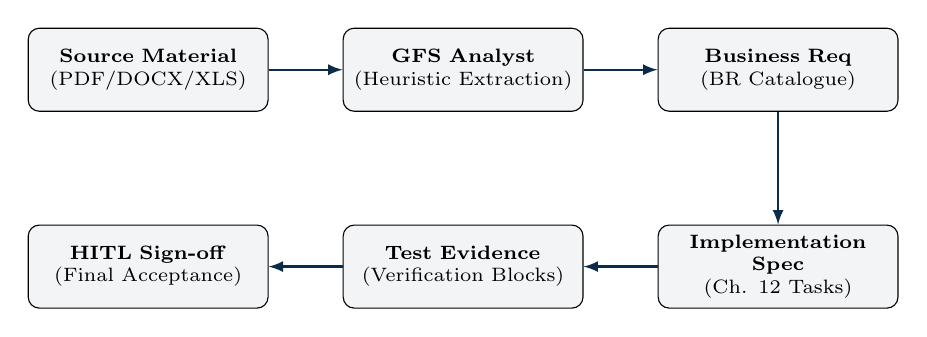
\begin{tikzpicture}[
node distance=1.5cm,
auto,
block/.style={rectangle, draw, rounded corners, fill=sapmidnight!5, text width=8em, text centered, minimum height=3em, font=\scriptsize},
arrow/.style={->, >=latex, thick, sapmidnight}
]
\node (source) [block] {\textbf{Source Material}\\(PDF/DOCX/XLS)};
\node (analyst) [block, right of=source, xshift=2.5cm] {\textbf{GFS Analyst}\\(Heuristic Extraction)};
\node (req) [block, right of=analyst, xshift=2.5cm] {\textbf{Business Req}\\(BR Catalogue)};
\node (spec) [block, below of=req, yshift=-1cm] {\textbf{Implementation Spec}\\(Ch. 12 Tasks)};
\node (test) [block, left of=spec, xshift=-2.5cm] {\textbf{Test Evidence}\\(Verification Blocks)};
\node (signoff) [block, left of=test, xshift=-2.5cm] {\textbf{HITL Sign-off}\\(Final Acceptance)};

\draw [arrow] (source) -- (analyst);
\draw [arrow] (analyst) -- (req);
\draw [arrow] (req) -- (spec);
\draw [arrow] (spec) -- (test);
\draw [arrow] (test) -- (signoff);
\end{tikzpicture}
\caption{The end-to-end compliance value stream.}
\end{figure}

\section{From PDF to Machine-Readable (YAML/JSON)}
The transformation from narrative prose to technical enforcement uses a semi-automated "Ground Truth" process. \cref{tab:artifact-linkage} maps the raw sources to their corresponding machine-readable counterparts.

\begin{table}[htbp]
\centering
\footnotesize
\caption{Source Material to Machine-Readable Linkage}
\label{tab:artifact-linkage}
\begin{tabularx}{\textwidth}{@{}l X X@{}}
\toprule
\textbf{Source Material (Raw)} & \textbf{Machine-Readable Artifact} & \textbf{Registry Location} \\
\midrule
\texttt{Accounts Payable DOI.docx} & \texttt{bh-ap-doi.json} & \texttt{structured/policies/} \\
\texttt{Saudi - OTP Entry...} & \texttt{ksa-vat-q3.yaml} & \texttt{structured/rules/} \\
\texttt{Specification Addendum} & \texttt{spec-addendum.yaml} & \texttt{arabic/machine-readable/} \\
\bottomrule
\end{tabularx}
\end{table}

\subsection{Extraction Methodology}
\begin{enumerate}
\item \textbf{Heuristic Extraction:} Initial requirement identification by GFS Analysts based on domain knowledge.
\item \textbf{Schema Normalization:} Mapping requirements to the \texttt{invoice.schema.json} and \texttt{vat-checklist.schema.json} defined in the technical spec.
\item \textbf{Formalization:} Converting narrative rules (e.g., "Full tax invoice must contain TIN") into JSON-Logic predicates for automated enforcement.
\end{enumerate}
\chapter{Business Requirements Catalogue}
\label{ch:requirements}

\begin{longtable}{p{2cm} p{5cm} p{7cm}}
\caption{Consolidated Business Requirements} \\
\toprule
\textbf{Req ID} & \textbf{Business Rule} & \textbf{Source Document Reference} \\
\midrule
\endfirsthead
\toprule
\textbf{Req ID} & \textbf{Business Rule} & \textbf{Source Document Reference} \\
\midrule
\endhead
\rowcolor{sapblue!5}
\textbf{BR-OCR-01} & Character precision for currency must exceed 99.5\%. & \texttt{Saudi - OTP Entry processing...} (p. 2) \\
\textbf{BR-VAT-SA} & Simplified vs Full Invoice determination based on 1000 SAR threshold. & ZATCA VAT Guidelines (Implicit in Saudi OTP) \\
\rowcolor{sapblue!5}
\textbf{BR-DOI-07} & Evidence-based seven-control sign-off for Bahrain. & \texttt{Accounts Payable DOI.docx} (Section 4) \\
\textbf{BR-TRN-01} & Translation must maintain semantic mapping for legal entity names. & \texttt{EDAA Annual Fee Invoice...} \\
\bottomrule
\end{longtable}
\chapter{Requirement-to-Specification Lineage}
\label{ch:lineage}

\begin{longtable}{p{2cm} p{6cm} p{6cm}}
\caption{Technical Traceability Matrix} \\
\toprule
\textbf{Req ID} & \textbf{Technical Implementation} & \textbf{Implementation Spec Ref} \\
\midrule
\rowcolor{sapamber!5}
\textbf{BR-OCR-01} & Confidence threshold calibration pilot. & \texttt{arabic-ap-spec} Ch. 10 \\
\textbf{BR-VAT-SA} & Rule ID \texttt{VAT-SA-SI-001} in VAT Engine. & \texttt{arabic-ap-spec} Ch. 8 \\
\rowcolor{sapamber!5}
\textbf{BR-DOI-07} & 28-state workflow wiring in \texttt{ap.workflow.advance}. & \texttt{arabic-ap-spec} Ch. 5 \& 6 \\
\textbf{BR-TRN-01} & Arabic--English translation gate calibration. & \texttt{arabic-ap-spec} Ch. 3 \\
\bottomrule
\end{longtable}

% --- NEW Detailed Analysis Chapters ---
\chapter{Source Analysis: Bahrain AP DOI}
\label{ch:analysis-bh-doi}

\section{Document Context}
The \texttt{Accounts Payable DOI.docx} (Bahrain) defines the delegation of authority and mandatory controls for invoice processing. This document was processed into \texttt{structured/policies/bh-ap-doi.json}.

\section{Detailed Requirement Mapping}

\begin{longtable}{p{5cm} p{5cm} p{5cm}}
\caption{Bahrain DOI: Source-to-Requirement Lineage} \\
\toprule
\textbf{Source Paragraph} & \textbf{Business Requirement} & \textbf{Formal Requirement (Spec)} \\
\midrule
\endfirsthead
\toprule
\textbf{Source Paragraph} & \textbf{Business Requirement} & \textbf{Formal Requirement (Spec)} \\
\midrule
\endhead
Section 4.1: ``All invoices must be matched against a valid Purchase Order prior to processing.'' & \textbf{BR-DOI-M1:} Mandatory PO-Matching for standard AP flow. & \texttt{arabic-ap-spec} Ch. 5 (PO-EPROC state machine). \\
\midrule
Section 4.2: ``Any variance > 5\% between PO and Invoice must be routed to the Finance Head.'' & \textbf{BR-DOI-V1:} Automated variance threshold detection. & \texttt{arabic-ap-spec} Ch. 6 (Variance Control C3). \\
\midrule
Section 4.7: ``The final payment file must be hashed and signed by two distinct personas.'' & \textbf{BR-DOI-S1:} Dual-Persona Cryptographic Sign-off. & \texttt{arabic-ap-spec} Ch. 12 (HITL Gate: Payment Instruction). \\
\bottomrule
\end{longtable}

\section{Machine-Readable Evidence (Fragment)}
The following YAML fragment was extracted from the DOI to drive the 28-state workflow engine:

\begin{lstlisting}[language=jsonx]
{
"policy_id": "BH-DOI-2026",
"controls": [
{
"id": "C3",
"description": "PO-Invoice Variance check",
"threshold": 0.05,
"escalation_persona": "finance_head"
}
]
}
\end{lstlisting}
\chapter{Source Analysis: Saudi VAT (ZATCA)}
\label{ch:analysis-sa-vat}

\section{Document Context}
The \texttt{Saudi - OTP Entry processing...} (ZATCA) defines the rules for electronic invoicing (E-Invoicing) and simplified vs. full tax invoice criteria. This was processed into \texttt{structured/rules/ksa-vat-q3.yaml}.

\section{Detailed Requirement Mapping}

\begin{longtable}{p{5cm} p{5cm} p{5cm}}
\caption{Saudi ZATCA: Source-to-Requirement Lineage} \\
\toprule
\textbf{Source Provision} & \textbf{Business Requirement} & \textbf{Technical Rule (Spec Ch. 8)} \\
\midrule
\endfirsthead
\toprule
\textbf{Source Provision} & \textbf{Business Requirement} & \textbf{Technical Rule (Spec Ch. 8)} \\
\midrule
\endhead
Article 53(b): ``Simplified Tax Invoices are issued for transactions < 1,000 SAR.'' & \textbf{BR-VAT-SI:} Determination of Simplified vs Full invoice based on threshold. & Rule \texttt{VAT-SA-THRESHOLD}: \texttt{gross\_amount < 1000} \\
\midrule
Article 54: ``Full Tax Invoices must display the Buyer's VAT Registration Number.'' & \textbf{BR-VAT-FULL:} Mandatory TRN/TIN field extraction for Full invoices. & Rule \texttt{VAT-SA-MANDATORY}: \texttt{exists(buyer.trn)} \\
\midrule
Phase 2 (ZATCA Integration): ``Invoice must contain a Phase-2 QR code including the ECDSA signature.'' & \textbf{BR-VAT-QR:} Extraction and verification of ZATCA QR signatures. & \texttt{arabic-ap-spec} Ch. 10 (OCR Pilot: QR calibration). \\
\bottomrule
\end{longtable}

\section{Machine-Readable Evidence (Fragment)}
The following YAML extraction defines the logic evaluated by the VAT engine for Saudi Arabian invoices:

\begin{lstlisting}[language=yamlx]
domain: "ksa-vat"
rules:
- id: "THRESHOLD_CHECK"
type: "classification"
predicate: "invoice.total_gross < 1000"
target_schema: "simplified_invoice"
- id: "TRN_CHECK"
type: "validation"
requirement: "buyer.trn must match ^3[0-9]{14}$"
\end{lstlisting}

% --- Incorporated Universal Chapters ---
\chapter{Global Wave-Dependency Manifest}
\label{ch:global-dependencies}

\section{Critical Path Visualization (Waves 1--3)}
The following chart defines the normative sequencing for implementation agents. A task in a later wave cannot be marked \textsc{complete} until its prerequisites in an earlier wave are validated.

\begin{figure}[htbp]
\centering
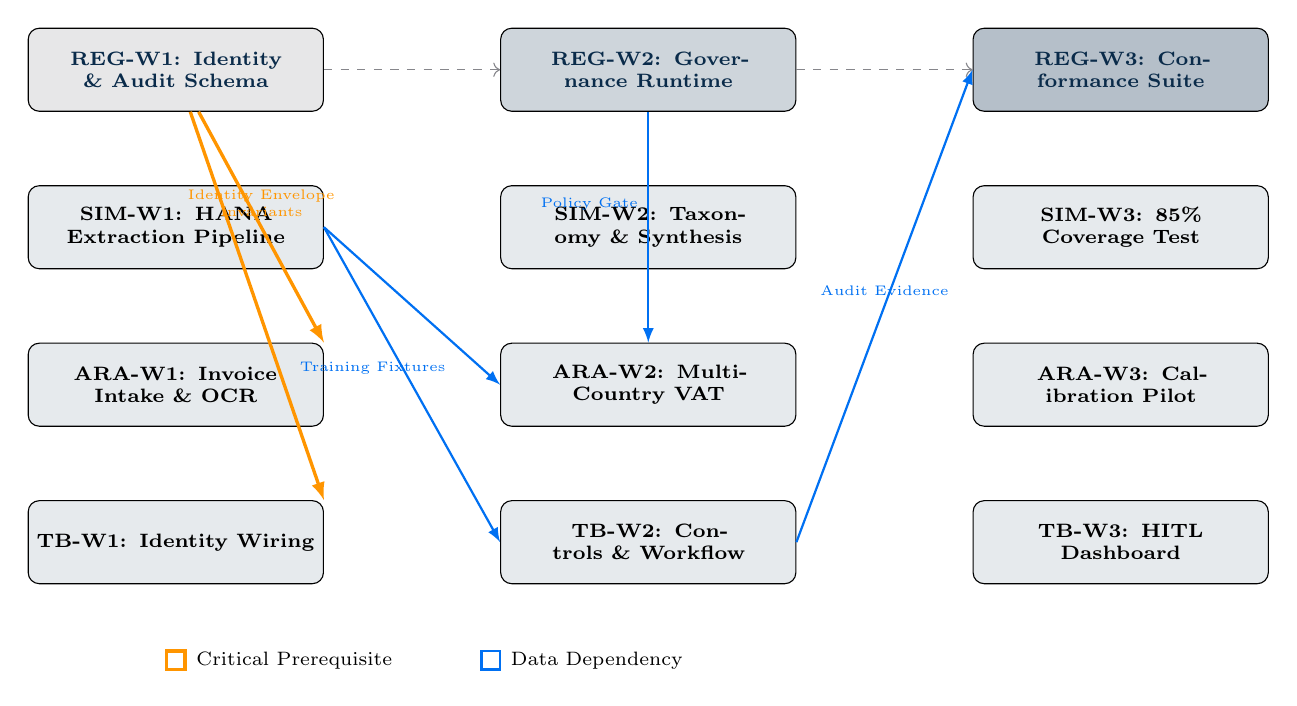
\begin{tikzpicture}[
node distance=1.5cm,
auto,
wavebox/.style={rectangle, draw, rounded corners, fill=sapmidnight!10, text width=10em, text centered, minimum height=3em, font=\scriptsize\bfseries},
dep/.style={->, >=latex, thick, sapblue},
critical/.style={->, >=latex, very thick, sapamber}
]
% --- Wave 1: Foundations ---
\node (r1) [wavebox, fill=sapgrey!20] {\textcolor{sapmidnight}{REG-W1: Identity \& Audit Schema}};
\node (s1) [wavebox, below of=r1, yshift=-0.5cm] {SIM-W1: HANA Extraction Pipeline};
\node (a1) [wavebox, below of=s1, yshift=-0.5cm] {ARA-W1: Invoice Intake \& OCR};
\node (t1) [wavebox, below of=a1, yshift=-0.5cm] {TB-W1: Identity Wiring};

% --- Wave 2: Core Build-out ---
\node (r2) [wavebox, right of=r1, xshift=4.5cm, fill=sapmidnight!20] {\textcolor{sapmidnight}{REG-W2: Governance Runtime}};
\node (s2) [wavebox, right of=s1, xshift=4.5cm] {SIM-W2: Taxonomy \& Synthesis};
\node (a2) [wavebox, right of=a1, xshift=4.5cm] {ARA-W2: Multi-Country VAT};
\node (t2) [wavebox, right of=t1, xshift=4.5cm] {TB-W2: Controls \& Workflow};

% --- Wave 3: Hardening ---
\node (r3) [wavebox, right of=r2, xshift=4.5cm, fill=sapmidnight!30] {\textcolor{sapmidnight}{REG-W3: Conformance Suite}};
\node (s3) [wavebox, right of=s2, xshift=4.5cm] {SIM-W3: 85\% Coverage Test};
\node (a3) [wavebox, right of=a2, xshift=4.5cm] {ARA-W3: Calibration Pilot};
\node (t3) [wavebox, right of=t2, xshift=4.5cm] {TB-W3: HITL Dashboard};

% --- Cross-Domain Dependencies (The Critical Path) ---
\draw [critical] (r1) -- node [above, font=\tiny, align=center] {Identity Envelope\\Invariants} (a1.north east);
\draw [critical] (r1) -- (t1.north east);
\draw [dep] (s1.east) -- node [above, font=\tiny, xshift=-0.5cm] {Training Fixtures} (t2.west);
\draw [dep] (s1.east) -- (a2.west);
\draw [dep] (r2.south) -- node [left, font=\tiny, yshift=0.3cm] {Policy Gate} (a2.north);
\draw [dep] (t2.east) -- node [above, font=\tiny] {Audit Evidence} (r3.west);

% --- Wave Transitions ---
\draw [->, dashed, sapgrey] (r1.east) -- (r2.west);
\draw [->, dashed, sapgrey] (r2.east) -- (r3.west);

% --- Legend ---
\node[draw, sapamber, very thick, label=right:\scriptsize Critical Prerequisite] at (0,-7.5) {};
\node[draw, sapblue, thick, label=right:\scriptsize Data Dependency, xshift=4cm] at (0,-7.5) {};

\end{tikzpicture}
\caption{Cross-specification dependency graph: The blueprint for platform rollout.}
\end{figure}

\section{Inter-Domain Prerequisite Matrix}

\begin{table}[htbp]
\centering
\footnotesize
\caption{Normative Cross-Domain Prerequisites.}
\label{tab:prerequisites}
\begin{tabularx}{\textwidth}{@{}l l l X@{}}
\toprule
\textbf{Target Task} & \textbf{Prerequisite} & \textbf{Ref ID} & \textbf{Rationale} \\
\midrule
\rowcolor{sapmidnight!5}
\textbf{ARA-W1} & REG-W1 (Identity) & \texttt{REG-IDENTITY-01} & Invoice intake must be audit-traced from Day 1. \\
\textbf{TB-W2}  & SIM-W1 (Extraction) & \texttt{SIM-EXTRACT-01} & Anomaly detection requires HANA schema metadata. \\
\rowcolor{sapmidnight!5}
\textbf{REG-W2} & SIM-W1 (Registry) & \texttt{SIM-REGISTRY-01} & Governance monitoring relies on the schema registry. \\
\textbf{ARA-W2} & REG-W2 (Pillar 1) & \texttt{REG-MGF-P1} & VAT release is an HITL gate governed by MAS Pillar 1. \\
\rowcolor{sapmidnight!5}
\textbf{TB-W3}  & ARA-W2 (Posted Invoices) & \texttt{ARA-AP-POST} & Review dashboard depends on posted AP data from Arabic domain. \\
\bottomrule
\end{tabularx}
\end{table}

\begin{adrbox}{Dependency Enforcement}
Implementation agents are strictly forbidden from "Fast-Forwarding" into Wave 2 if Wave 1 critical prerequisites (marked in \textcolor{sapamber}{\textbf{Gold}}) are in a \textsc{gap} or \textsc{partial} state.
\end{adrbox}



\end{document}
